% 固定来源 PDF 第 21 题原图结构示意重绘（扫描件无可解析内容流，按原页关系重绘）。
% 两平面相交于 l，矩形 ABCD 在 alpha 内，P 在 beta 内且 PA 垂直 alpha；投影不表示度量比例。
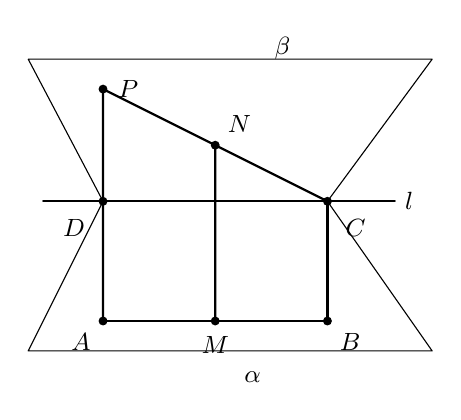
\begin{tikzpicture}[scale=.95,font=\small,line cap=round,line join=round]
  \coordinate (D) at (1.2,0);
  \coordinate (C) at (4.2,0);
  \coordinate (A) at (1.2,-1.6);
  \coordinate (B) at (4.2,-1.6);
  \coordinate (P) at (1.2,1.5);
  \coordinate (M) at (2.7,-1.6);
  \coordinate (N) at (2.7,0.75);
  % 两平面（相交于 l）
  \draw[thin] (D)--(C)--(5.6,-2.0)--(0.2,-2.0)--cycle;
  \draw[thin] (D)--(C)--(5.6,1.9)--(0.2,1.9)--cycle;
  \draw[thick] (0.4,0)--(5.1,0) node[right] {$l$};
  \node at (3.2,-2.35) {$\alpha$};
  \node at (3.6,2.05) {$\beta$};
  % 矩形与给定线段
  \draw[thick] (A)--(B)--(C)--(D)--cycle;
  \draw[thick] (P)--(A) (P)--(C) (M)--(N);
  % 标签
  \fill (A) circle (1.7pt) node[below left=1pt] {$A$};
  \fill (B) circle (1.7pt) node[below right=1pt] {$B$};
  \fill (C) circle (1.7pt) node[below right=3pt] {$C$};
  \fill (D) circle (1.7pt) node[below left=3pt] {$D$};
  \fill (P) circle (1.7pt) node[right=2pt] {$P$};
  \fill (M) circle (1.7pt) node[below=2pt] {$M$};
  \fill (N) circle (1.7pt) node[above right=1pt] {$N$};
\end{tikzpicture}
